\section{Local CA Signing The X.509 Certificate}

As evident by figure \ref{fig:x509_creation:ca}, we created our local certificate of authority with the basic constraint generation command. This certificate was filled in with similar details in figure \ref{fig:x509_creation:jason}, however the first and last name was `Antonio Gargaro'. We then signed our own X.509 certificate with the command at the top of figure \ref{fig:ca_sign:ca_sign_x509}.

\begin{figure}[hbt!]
	\centering
	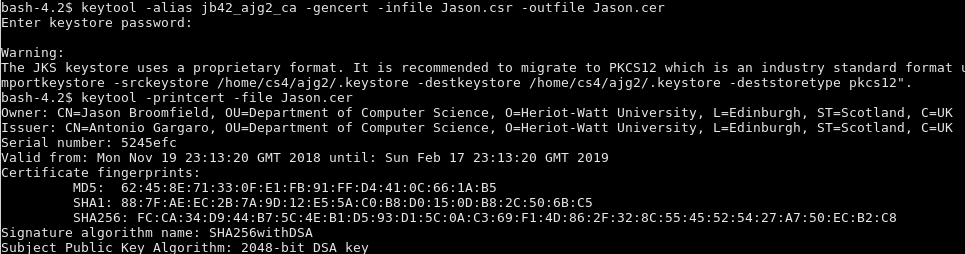
\includegraphics[width=\textwidth]{imgs/x509_creation/x509_Signed_By_CA.PNG}
	\caption{Signing X.509 with our local Certificate Authority}
	\label{fig:ca_sign:ca_sign_x509}
    \noindent\makebox[\linewidth]{}
\end{figure}
